\section{Python Exercise: Two-Channel Delay Recovery}\label{sec:p8}

\begin{figure}[htbp]
	\centering
	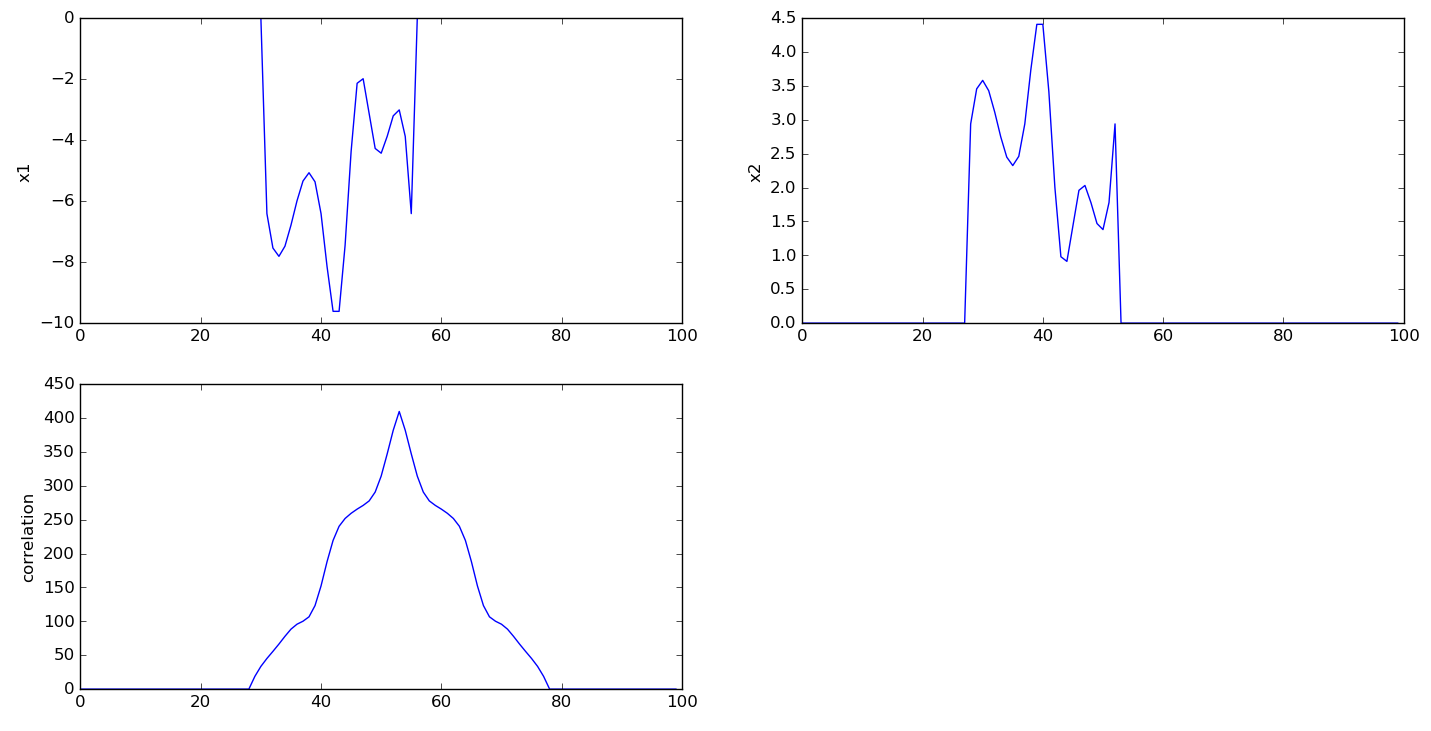
\includegraphics[width=\textwidth]{images/p8-1}
	\caption{An output of two-channel delay recovery. The top 2 images are $x_1$ and $x_2$, where the third one is their cross-correlation.}
	\label{fig:p8-1}
\end{figure}

Figure \ref{fig:p8-1} shows an the generated signals and their cross-correlation. The output of the code is:

\begin{lstlisting}
delta=-3, rho=-2.1807
n2=27, n1=30, n2-n1=-3
alpha1=-1.0682, alpha2=0.4899, alpha1/alpha2=-2.1807
\end{lstlisting}